%% -------------------------------------
% Creates the front matter (title page(s), abstract, list of papers)
%% -------------------------------------
\frontmatterCS
 
%% Optional dedication
%\dedication{Pour {\Papa}, {\Maman}, {\Franck} et {\Alexandre}}

%% List of papers
\listofpapersintro{This thesis is based on the following papers, which are referred in the text by their roman numerals.}% 
%\listofpapersoutro{Reprints were made with permission from the publishers.}

\newcommand{\conference}[1]{\marginpar{\tikz[baseline=(c.base)]\node(c)[conference]{#1};}}

% Environment used to create a list of papers
\begin{listofpapers}
  %
  \item \label{paper:ATVA'13}%
    {\bf Verification of Heap Manipulating Programs with
Ordered Data by Extended Forest Automata} %{\small (Parameterized Verification through View Abstraction)}}
    \conference{ATVA'13}
    \\{\footnotesize Parosh Aziz Abdulla, Lukáš Holík, Bengt Jonsson, Ondřej Lengál, Cong Quy Trinh, Tomáš Vojnar}.
    \\In {\it Automated Technology for Verification and Analysis}, 2013.
    % 
  \item \label{paper:SAS16}%
    {\bf Automated Verification of Linearization Policies}\conference{SAS'16}
   % \\{\bf for Highly Concurrent Data Structures}
    \\{\footnotesize Parosh Aziz Abdulla, Bengt Jonsson, and Cong Quy Trinh}.
    \\In {\it Tools and Algorithms for the Construction and Analysis of Systems}, 2016.
    
    \item \label{paper:ESOP18}%
    {\bf Fragment Abstraction for Concurrent Shape Analysis
}\conference{ESOP'18}
   % \\{\bf for Highly Concurrent Data Structures}
    \\{\footnotesize Parosh Aziz Abdulla, Bengt Jonsson, and Cong Quy Trinh}.
    \\In {\it European Symposium on Programming}, 2018.
     % 
\end{listofpapers}


%% Tack Parosh!
%\chapter[Acknowledgements = Thank you \Parosh !]{Acknowledgements}
\chapter*{Acknowledgements} 
%\addcontentsline{toc}{chapter}{Acknowledgements\texorpdfstring{~(= Thank you, \Parosh !)}{}}
%
%I have only two words to describe how I feel: {\Chalk Tack Parosh!}
%
%\bigskip
%\noindent%
%Turn the page to see what I mean.
%% I'm showing on the next two pages how I would like to write this
%% section.
%%\index{Acknowledgements}
%\index{Acknowledgements!Thank You, {\Chalk Parosh}}
%
%\def\Paroshshape{%
{20}%
%% P %%%%%%%%%%%%%%%%%%%%%%%%%%%%%%%%%%%%%%%%%%%%%%%%%%%%%%%%%%%%%%%%
{0}b{0}\\%
{0}t{0}{40}\\%
{5}t{0}{40}\\%
{5.01}t{17}{6}st{34}{6}\\% 
{9.99}t{17}{6}jt{34}{6}\\% 
{10}t{17}{23}\\% 
{15}t{23}{11}\\%
{15}e{34}\\%
%% A %%%%%%%%%%%%%%%%%%%%%%%%%%%%%%%%%%%%%%%%%%%%%%%%%%%%%%%%%%%%%%%%
{17}b{0}\\%
{17}t{0}{34}\\%
{22}t{0}{40}\\%
{22.01}t{17}{6}st{34}{6}\\%
{26.99}t{17}{6}jt{34}{6}\\%
{27}t{0}{40}\\%
{32}t{0}{34}\\%
{32}e{34}\\%
%% R %%%%%%%%%%%%%%%%%%%%%%%%%%%%%%%%%%%%%%%%%%%%%%%%%%%%%%%%%%%%%%%% 
{34}b{0}\\%
{34}t{0}{34}\\%
{39}t{0}{40}\\%
{39.01}t{16}{5}st{34}{6}\\%
{43.99}t{0}{22.5}jt{34}{6}\\%
{44}t{0}{40}\\%
{44.01}t{0}{17.5}st{17.5}{22.5}\\%
{49}t{0}{0}t{23}{11}\\%
{49}e{34}\\%
%% 0 %%%%%%%%%%%%%%%%%%%%%%%%%%%%%%%%%%%%%%%%%%%%%%%%%%%%%%%%%%%%%%%% 
{51}b{6}\\%
{51}t{6}{28}\\%
{56}t{0}{40}\\%
{56.01}t{0}{10}st{30}{10}\\%
{58}t{0}{6}t{34}{6}\\%
{60.99}t{0}{10}jt{30}{10}\\%
{61}t{0}{40}\\%
{66}t{6}{28}\\%
{66}e{34}\\%
%% S %%%%%%%%%%%%%%%%%%%%%%%%%%%%%%%%%%%%%%%%%%%%%%%%%%%%%%%%%%%%%%%% 
{68}b{0}\\%
{68}t{0}{6}t{23}{11}\\%
{73}t{0}{6}t{17}{23}\\%
{73.01}t{0}{6}t{17}{6}st{34}{6}\\%
{77.99}t{0}{6}jt{17}{6}t{34}{6}\\%
{78}t{0}{23}t{34}{6}\\%
{83}t{6}{11}t{34}{6}\\%
{83}e{40}\\%
%% H %%%%%%%%%%%%%%%%%%%%%%%%%%%%%%%%%%%%%%%%%%%%%%%%%%%%%%%%%%%%%%%% 
{85}b{0}\\%
{85}t{0}{40}\\%
{90}t{0}{40}\\%
{90.01}t{17}{6}\\% 
{94.99}t{17}{6}\\% 
{95}t{0}{40}\\% 
{100}t{0}{40}\\%
{100}e{40}%
}

\def\Tackshape{%
{20}%
%% T %%%%%%%%%%%%%%%%%%%%%%%%%%%%%%%%%%%%%%%%%%%%%%%%%%%%%%%%%%%%%%%%
{0}b{32}\\%
{0}t{32}{8}\\%
{6}t{32}{8}\\%
{6.01}t{0}{40}\\% 
{10.99}t{0}{40}\\% 
{11}t{32}{8}\\% 
{17}t{32}{8}\\%
{17}e{40}\\%
%% A %%%%%%%%%%%%%%%%%%%%%%%%%%%%%%%%%%%%%%%%%%%%%%%%%%%%%%%%%%%%%%%%
{19}b{0}\\%
{19}t{0}{34}\\%
{24}t{0}{40}\\%
{24.01}t{17}{6}st{34}{6}\\%
{28.99}t{17}{6}jt{34}{6}\\%
{29}t{0}{40}\\%
{34}t{0}{34}\\%
{34}e{34}\\%
%% C %%%%%%%%%%%%%%%%%%%%%%%%%%%%%%%%%%%%%%%%%%%%%%%%%%%%%%%%%%%%%%%% 
{36}b{6}\\%
{36}t{6}{28}\\%
{41}t{0}{40}\\%
{41.01}t{0}{10}st{30}{10}\\%
{46}t{0}{6}t{34}{6}\\%
{51}t{3}{6}t{31}{6}\\%
{51}e{37}\\%
%% K %%%%%%%%%%%%%%%%%%%%%%%%%%%%%%%%%%%%%%%%%%%%%%%%%%%%%%%%%%%%%%%% 
{53}b{0}\\%
{53}t{0}{40}\\%
{58}t{0}{40}\\%
{58.01}t{15}{10}\\% 
{63.99}t{0}{40}\\% 
{64}t{0}{17}st{23}{17}\\% 
{69}t{0}{6}t{34}{6}\\% 
{69}e{40}%
}
 %% Defines Parosh and Tack shapes
%
%
%\newpage
%\noindent%
%{\footnotesize
%\shapepar\Paroshshape%
%FINALLY! It has been long and even tough at times, but I made it!
%%
%We all know that I would not be writing this section if Parosh had not
%been there. I hope he understands how grateful I am to count him as my
%supervisor. But let me save the best for last and
%%
%let me start by thanking everyone else who contributed to my journey
%that leads to this thesis. I must of course start with my favorite
%czech companion \lukas. \lukasshort\ is a great researcher with
%tremendous motivation and skills. He was patient to listen to my
%ideas, which we both know must first make their way through a thick
%layer of verbose ramblings. It is nevertheless a great pleasure to
%work with him.
%%
%I enjoyed extremely much working with \bengt, and I wish we had more
%projects in common. He made me quickly feel at ease and confident,
%even though I felt intimidated at first. This was really impressive to
%witness such a great mind at work.
%% 
%I would like to thank \noomene, \ahmed, Lisa Kaati, Mayank Saksena,
%Johan Deneux, Sven Sandberg during my early days as a PhD student and
%%
%lately \jonathan, Othmane Rezine, Faouzi Atig, Trinh Cong Quy, Carl
%Leonardsson, Jari Stenman, Yunyun Zhu and Muneeb Khan.
%%
%From outside the IT department of Uppsala University, I would like to
%mention Tomas Vojnar, Yu-Fang Chen and Giorgio Delzanno who showed me
%how research works in other universities and how lucky I was at
%Uppsala University with Parosh.
%%
%From Uppsala University, my deepest thank you goes to Ivan
%Christoff. Ivan seems to always %genuinely
%have our well-being at heart. It is a truly remarkable quality that
%leaves me with a profond gratitude. %
%I would like to thank Mats Daniels, Wang Yi, Joachim Parrow, Ulrika
%Jaresund, Ulrika Andersson, Mattias Wigberg, Karl Marklund, to always
%have the time to lend me a hand or a complicit hear. %
%%
%%Everybody else at the department that I meet from time to time %
%%
%A special note goes to my previous supervisors Björn Victor and Erik
%Hagersten who introduced me to the PhD program.
%%
%%
%\par
%}
%
%\newpage
%\noindent%
%{\small%\footnotesize
%\shapepar\Tackshape%
%%
%I developed a special profile as a PhD student, since I was given the
%chance to be the main teacher of several courses. Thank you Mats for
%trusting me with it. This was way more fun and challenging than a
%teaching assistant position.
%%
%Along with teaching skills, I also had the opportunity to learn a lot
%culturally about Sweden. This is mainly due to my participation in
%local dance schools. First as a student (thank you Johanna Berglund to
%drag me into that world) and then as a teacher. Yes, you read it
%right, I am a dancing nerd.  So it is now time to mention everyone
%else who contributed to my special time in Sweden. This time is
%probably not over but I still want to thank them. So here I
%shoot.
%%
%In Uppsala, thank you Junior, Marina, Fabien, Chris, Sepideh, Paul,
%Camilla, Paola, Lilly, Lina, Carlos, Alexander~K, Patrick, Alexander~H,
%Alexander~Ki, Linda, Yuri, Lisa~K, Tanja, Anna~G, Lisa-Marie, Ronak,
%Sasha, Amanda, Annika, Becky, Eva, Carmen, Eva-Lena, Wendelin, Isabel,
%John, Maele, Maggie, Maria, Malou, Rebecca, Tim, Anna~C, Erik~I,
%Matilda, Tove, Mia, Erika and Chiqui.
%%
%Special thanks to my tennis partners Nadim and Sebastian.
%%
%In Stockholm, thank you Kristofer, Marina, Alexander, Adela, Mina,
%Andreas, Behnaz, Egle, Camilla~C, Eshtar, Hind, Jaime, Jennifer,
%Johanna~E, Lalla, Pascal, Tofik and everyone else that I will soon meet.
%%
%And of course, let's not forget Lisa and Liza.
%%
%So, finally, we come to the main acknowledgment. This thesis starts
%with Parosh on my side and I would like to finish that section
%with {\parosh}. This has not been easy and despite my stubbornness, he
%was willing to put efforts into helping me. He backed me up at
%difficult times and trusted me at some other times. He gave me a
%chance to travel, trusted me with conference presentations and showed
%me that I maybe know more than it looked like.
%%
%It is almost too good to be true. Thank you {\Parosh}.
%\par
%}


%% Summaries in Swedish and French
\cleardoublepage
\addcontentsline{toc}{chapter}{Summary} 
%%% =============================================================
%\chapter*{Sammanfattning på Svenska \texorpdfstring{\hfill\raisebox{-2em}{
\includegraphics[height=3em]{img/sverige.png}}}{}}
%\addcontentsline{toc}{section}{\texorpdfstring{\protect\raisebox{-0.5ex}{\protect\makebox[3ex]{\protect
\includegraphics[height=1em]{img/flag-sverige.png}}}}{} in Swedish}
%\index{Summary!Sammanfattning \protect\makebox[3ex]{\protect
\includegraphics[height=1em]{img/flag-sverige.png}}}
%
%Du har säkerligen använt en dator och varit väldigt nöjd, och detta
%för att den förenklade många långa och svåra %mödosamma
%uppgifter.
%%
%Ibland gör den dock inte som du vill: du klickar på knappen ``Gör
%det'', men den följer inte ditt kommando. Eller ännu värre, datorn
%hänger upp sig och svarar inte på något kommando alls.
%%
%Viktiga arbetstider har kanske gått till spillo.
%%
%Du tar ett djupt andetag, startar om datorn, och allting fungerar igen
%som det ska.
%%
%Felet verkar komma från \emph{programvaran} som styr datorn, inte från
%själva maskinen.
%%
%Du undrar varför detta fel inte redan korrigerats, och dessutom,
%varför det från början inte \emph{försäkrades} om att felet inte kunde
%inträffa.
%
%
%Termen \emph{buggar} används generellt för att beskriva alla typer av
%fel, vare sig felet finns i dem elektriska delarna av maskinen eller i
%programmeringen.
%%
%Med tanke på hur komplexa dagens datorer är, är det inte förvånande
%att de innehåller många buggar.
%%
%De behöver ju %faktiskt
%hantera en stor mängd parametrar och egenskaper som kan generera
%% ge plats till
%många olika möjliga beteenden.
%%
%Och vi nämner inte ens den mänskliga faktorn som inför fel under
%programmeringsfasen!
%%
%Därför finns det en trend att bygga datorer med flera mindre enheter,
%som då gör datorn enklare att hantera.
%%
%Men då ställs vi inför ett nytt problem: dessa enheter kan när som
%helst kommunicera med varandra.
%%
%På grund av denna oförutsägbarhet blir det väldigt svårt att ta hänsyn
%till alla scenarier.
%
%Företag som tillverkar programvara har inget intresse av att lämna
%buggar, eftersom ett fel någonstans kan orsaka en rad andra fel i
%efterhand. %kaskad
%%
%De inkluderar därför en viktig kvalitetskontroll under
%utvecklingsfasen: om det finns för många buggar blir det helt enkelt
%inte kostnadseffektivt eller ens möjligt att senare eliminera dem.
%%
%En del buggar är dock enklare att lösa än andra.
%%
%Det spelar faktiskt ingen större roll om man inte kan svara i
%telefonen när man får ett samtal, eller om texteditorn förlorar dem
%senaste dokumentsuppdateringarna.
%%
%Detta är väldigt tråkigt, men ingen fara på taket! Vi klarar oss och
%väntar bara på programuppdateringen som löser buggen.
%%
%Å andra sidan får inga fel inträffa för dem så-kallade %
%\emph{kritiska systemen}, vars säkerhet är viktig i allra högsta
%grad. Alla fel måste elimineras, antingen i programvaran eller i
%maskinvaran.
%%
%Det är oacceptabelt, till exempel, att en pacemaker slutar fungera när
%ägaren passerar säkerhetskontrollen på flygplatsen, att krockkudden
%inte utlöses snabbt nog vid en trafikolycka om radion är på, eller om
%två tåg kolliderar på grund av att signalsystemet inte fungerat.
%%
%Därför är det nödvändigt att utveckla metoder som upptäcker
%ett felaktigt beteende i sådana system.
%
%
%Den vanligaste metoden är \emph{testing}: man kör programmet med olika
%värden för varje variabel och kollar om funktionaliteten
%överensstämmer med det som förväntas.
%%
%Dessa testscenarier är genomtänkta för att beskriva ett maximalt antal
%beteenden.
%%
%När komplexiteten däremot ökar, kan programmet befinna sig i väldigt
%många olika tillstånd. Det börjar då bli svårt att \emph{garantera}
%att metoden täcker alla möjliga programkörningar.
%%
%Det är även rent av omöjligt om systemet innehåller en parameter vars
%värde exempelvis är en siffra.
%%
%Metoden är ett effektivt sätt att upptäcka enkla buggar snabbt, men
%subtila buggar, såsom dem som kommer från en oförutsägbar tajming,
%kvarstår obemärkta.
%%
%För dem kritiska systemen där säkerheten är ytterst viktig, är det
%otänkbart att använda en metod som eventuellt tar sig igenom alla
%tester, men fortfarande innehåller buggar.
%
%För att visa att ett program verkligen uppfyller vissa egenskaper,
%måste vi först komma överens om vad det ska överensstämma med
%---vilket formellt heter en \emph{specifikation}.
%%
%Genom att lista programkonfigurationerna som borde undvikas, eller som
%önskas, alternativt båda, så beskriver man dem två kategorierna av
%specifikationer: \emph{säkerhetsegenskaper} och
%\emph{livlighetsegenskaper} (Safety och Liveness på engelska).
%%
%Till exempel, ``pacemakern stannar aldrig'', ``krockkudden måste
%öppnas inom mindre än $x$~millisekonder'', eller ``ingen enstaka
%process blockerar övriga processer'' är säkerhetsegenskaper.
%%
%Vi måste se till att programmet aldrig befinner sig i en felaktig
%konfiguration.
%% 
%Till motsatsen, ``brevbäraren levererar till rätt mottagare'',
%``systemet gör framsteg'', eller ``servern hanterar en HTTP-förfråga''
%är livlighetsegenskaper, där man observerar rätta konfigurationer,
%förknippade med vissa sannolikheter.
%% 
%Det är upp till oss att definiera vad specifikationen ska innehålla, för
%att verifiera det som önskas.
%% 
%Om ett låsningsfritt bromssystem (ABS) % Antilock Braking System
%beräknar hur hårt bilens bromsning ska vara men gör detta för sent,
%bör systemet beträktas som felaktigt.
%% 
%Denna avhandling fokuserar på säkerhetsegenskaper.
%\begin{statement}
%  {\bf Säkerhet}: %
%  {\it Givet en specifikation, kan systemet hamna i en fel konfiguration?}
%\end{statement}
%
%%% ------------------------
%Snarare än att testa programmet i specifika scenarier eller att
%analysera källkoden, fokuserar vi i denna avhandling på \emph{formell
%  verifiering}, som är ett matematiskt ramverk, för att \emph{bevisa}
%att programmet uppfyller sina egenskaper.
%
%Dessutom vill vi bevisa det helt \emph{automatiskt}, det vill säga
%utan tillsyn av användaren.
%%
%Vi börjar genom att extrahera en modell som motsvarar det ursprungliga
%programmet. I samband med det borttar vi delarna som är irrelevanta
%för den egenskapen som verifieras.
%%
%Men vad händer när programmet manipulerar obegränsade variabler? Vi
%talar då om system med ett oändligt antal tillstånd, och vi behöver
%framställa en approximation som är i linje med själva programmet.
%%
%Målet är att utforma en metod som \emph{garanterar} att inget fel
%kvarstår, och som även ger svar inom en rimlig tid.
%
%Många system med ett oändligt antal tillstånd kan faktiskt
%karakteriseras av en familj som består av system med ett ändligt antal
%tillstånd, och en parameter (eller flera) med värde från en obegränsad
%domän.
%%
%För varje värde på parametern, innehåller systemet ett ändligt antal
%tillstånd.
%%
%Parametern kan exempelvis vara
%antalet processer som är aktiva i en viss session av ett protokoll, %
%antalet noder i ett nät, %
%eller hur komponenterna av ett program kommunicerar med varandra.
%%
%Hur som helst, system som innehåller en preliminärt okänd parameter
%bör ha ett korrekt beteende oavsett värdet på parametern. De betraktas
%därför som system med ett oändligt antal tillstånd och kallas för
%parametriserade system.
%I denna avhandling presenterar vi två metoder för att verifiera vissa
%säkerhetsegenskaper hos sådana parametriserade system.
%
%Den första metoden körs baklänges. Den startar från dem felaktiga
%tillstånden, och beräknar vilka andra tillstånd som skulle kunna leda
%till ett fel.
%%
%Med andra ord upptäcker metoden alla konfigurationer som direkt eller
%indirekt är felaktiga.
%%
%Om initialtillstånden av programmet inte tillhör dem sistnämnda, anses
%programmet vara korrekt. Vi måste såklart först se till att
%approximationen av modellen motsvarar det ursprungliga programmet.
%
%Den andra metoden startar från initialtillstånden. Den begränsar sig
%till små värden av parametern, och härleder ett tröskelvärde, efter
%vilket metoden inte behöver fortsätta: den har faktiskt all nödvändig
%information för att dra slutsatsen att det inte finns några
%felkonfigurationer för större värden på parametern över denna tröskel.
%% 
%För att förenkla, bryter metoden ner varje konfiguration i små bitar
%av en viss storlek, och rekombinerar bitarna på alla möjliga sätt,
%just för att skapa konfigurationer av större storlek (litegrann som
%Lego\-bitar). %tegelstenar
%% 
%Tanken är att samla alla dem små bitarna och se till att ingen
%rekombination matchar någon felaktig konfiguration.
%% 
%I så fall är tröskeln hittad. Annars börjar man om med lite större
%bitar.
%
%
%Slutligen är det intressant att undra vilka av villkoren som behövs
%för att metodens beräkningar inte ska fortsätta för evigt. Problemet
%klassas som oavgörbart, det vill säga att det inte finns någon
%generell metod som kan lösa \emph{alla} instanser av
%problemet. Däremot har dessa två metoder trots allt visat sig vara
%väldigt effektiva.
%%
%Där andra metoder tog timmar, kunde dessa två metoder faktiskt
%verifiera vissa program inom sekunder, vilket var målet.
%%
%I vissa fall kan man även ge garanti på att antalet beräkningar är
%begränsad.
%

%%% =============================================================
%\chapter*{Résumé en Français \texorpdfstring{\hfill\raisebox{-1em}{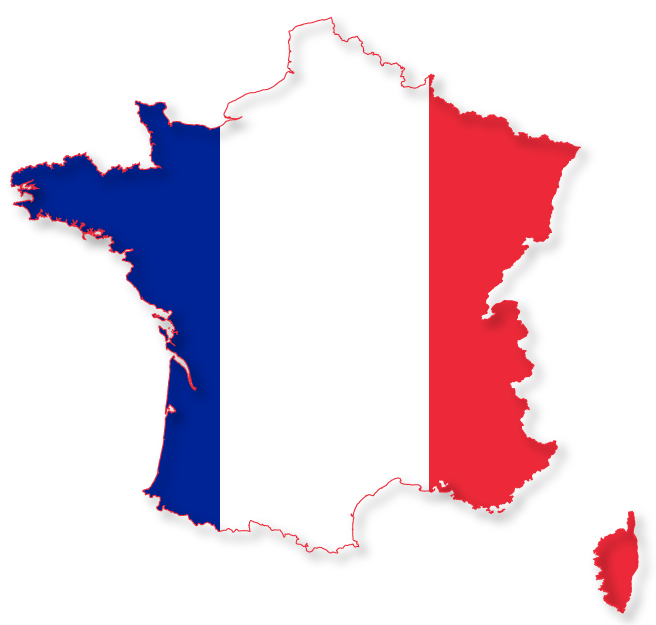
\includegraphics[height=2em]{img/france.png}}}{}}
%\addcontentsline{toc}{section}{\texorpdfstring{\protect\raisebox{-0.5ex}{\protect\makebox[3ex]{\protect
\includegraphics[height=1em]{img/flag-france.png}}}}{} in French}
%%% =============================================================
%%\index{Summary!en français}
%%\index{Summary!en français \protect\makebox[3ex]{\protect
\includegraphics[height=1em]{img/flag-france.png}}}
%\index{Summary!Résumé \protect\makebox[3ex]{\protect
\includegraphics[height=1em]{img/flag-france.png}}}
%
%Pour vous simplifier beaucoup de tâches longues et ardues, vous avez
%certainement déjà utilisé un ordinateur et en étiez très satisfaits.
%% 
%Cependant, de temps à autre, l'ordinateur ne fait pas ce que vous lui
%demandez: vous cliquez sur le bouton ``Faire ça'' et il ne le fait
%pas. Ou pire, l'ordinateur se bloque et ne répond plus à aucune
%commande. D'importantes heures de travail viennent peut-être de
%s'envoler.
%% 
%Vous gardez votre sang-froid, redémarrer l'ordinateur et tout semble à
%nouveau marcher comme prévu.
%% 
%L'erreur ne vient visiblement pas de l'ordinateur lui-même, mais elle
%semble venir du \emph{logiciel} qui contrôle ce dernier.
%% 
%Vous vous demandez pourquoi cette erreur n'a pas été corrigée, et qui
%plus est, pourquoi on ne s'est pas \emph{assuré} dès le départ que
%l'erreur ne survient pas. %survient
%
%Les différentes composantes électriques de la machine peuvent tomber
%en panne. Historiquement, ces erreurs sont appelées des \emph{bugs} %
%-- le terme anglais pour cafards -- %,
%car il est dit qu'un vrai cafard est entré un soir dans le châssis
%d'une machine qu'un informaticien fabriquait dans son garage,
%détruisant au passage quelques morceaux du circuit électrique. En se
%réveillant le lendemain, il s'est rendu compte que la machine
%manifestait un comportement bizarre.  Le terme est resté et est
%maintenant utilisé pour qualifier toutes sortes d'erreurs de
%programmation en général.
%% , c'est-à-dire quand un programme ne
%% solutionne pas le problème donné.
%
%Étant donné la complexité des ordinateurs de nos jours, il n'est pas
%étonnant qu'ils soient sujets à de nombreuses erreurs.
%% 
%Ils nécessitent de prendre en charge une multitude de
%paramètres, %et de caractéristiques,
%sans oublier les erreurs humaines introduites lors de la phase de
%programmation.
%% 
%C'est pourquoi %il est préférable
%la tendance est %
%de construire ces machines en composant plusieurs unités plus
%réduites.
%% 
%Chaque unité est de ce fait plus facile à contrôler, mais
%ces unités peuvent communiquer les unes avec les autres à n'importe
%quel moment.
%% 
%Il devient alors très difficile de prendre en compte tous les
%scénarios possibles et de prédire le comportement général du
%programme, à cause de ce caractère imprévisible. % hasardeux
%
%Les entreprises fabriquant ces logiciels n'ont pas intérêt à y laisser
%des bugs, puisqu'une erreur %quelque part
%peut engendrer d'autres erreurs en cascade.
%% 
%Celles-ci passent du temps, et de l'argent, à traquer ces bugs et s'il
%y en a trop, il n'est simplement plus rentable ou même envisageable de
%les éliminer.
%% 
%Les entreprises mettent donc en place, dans le cycle de développement de
%chaque projet, une phase essentielle de contrôle de qualité.
%% 
%Cela dit, certains bugs sont plus urgents à résoudre que d'autres.
%% 
%Ce n'est pas très grave si on ne peut pas décrocher son téléphone lors
%d'un appel, ou si l'éditeur de texte perd les derniers ajouts à notre
%document. C'est peut-être très ennuyeux mais le pronostic vital n'est
%pas engagé! On s'en remettra, en attendant la mise à jour du logiciel
%incriminé.
%% 
%Par contre, ce n
%'est pas le cas pour ces systèmes, dits
%\emph{critiques}, pour lesquels la sûreté est primordiale. Toutes les
%erreurs doivent être éliminées, qu'elles soient au niveau logiciel ou
%au niveau de la machine.
%% 
%Il n'est pas acceptable, par exemple, qu'un pacemaker s'arrête de
%fonctionner quand on passe le portique dans le métro, que l'avion
%parte en chute libre quand l'équipage allume le signal d'interdiction
%de fumer à bord, ou encore que deux trains entrent en collision parce
%que les feux ont mal fonctionné.
%% 
%% C'est pourquoi 
%Il est nécessaire de concevoir des techniques pour détecter ce genre
%d'erreurs.
%
%Pour améliorer la qualité des logiciels, il existe une technique
%prédominante: la méthode qui vise à soumettre le programme à une série
%de \emph{tests} et d'en observer les résultats.
%% 
%Ces scénarios de tests sont soigneusement conçus afin de couvrir un
%maximum d'exécution possible du programme.
%% 
%Dans la même catégorie, il est possible d'extraire un \emph{modèle} du
%programme %
%% , en prenant soin d'éliminer les morceaux superflus pour les
%% tests en cours, et 
%et de l'utiliser pour \emph{simuler} le programme.
%% 
%Cela dit, lorsque le programme est de plus en plus grand et complexe,
%que l'on utilise un modèle ou le programme lui-même, il devient
%impossible de \emph{garantir} que toutes les exécutions soient prises
%en compte par une batterie de scénarios.
%% 
%C'est même tout bonnement impossible lorsque le programme contient un
%paramètre qui varie sur un domaine non borné, comme par exemple, un
%entier.
%% 
%Ces deux méthodes sont utiles pour découvrir rapidement de simples
%erreurs, mais les erreurs subtiles, comme celles concernant le timing,
%restent non détectées.
%% 
%Dans le cas des systèmes qui requièrent une sûreté maxi\-male, il
%n'est pas concevable d'utiliser un programme qui pourrait contenir une
%erreur, quand bien même il ait passé tous ses tests.
%
%Comment donc s'assurer que toutes les exécutions d'un programme aient
%été prises en compte?
%% 
%On ne peut certainement pas faire tourner le programme et se contenter
%d'un ensemble restreint d'exécutions ou de valeurs pour les paramètres
%du programme.
%% 
%La technique d'\emph{analyse statique} offre une couverture complète
%d'un programme, sans l'exécuter. Elle inspecte toutes les exécutions
%\emph{faisables}, c'est-à-dire celles que le programme \emph{peut}
%effectuer et non celles qu'il \emph{va} effectuer.
%% 
%Le code source du programme y est sous la loupe, qu'il soit lisible
%par un humain ou seulement par une machine.
%% 
%Chaque combinaison est prise en compte ce qui rend cette méthode
%rapidement ingérable.
%% On pourrait être moins naïf, et se limiter à
%% certaines parties du code qui peuvent contenir les erreurs. Cependant,
%% déterminer leur emplacement est certainement aussi difficile que de
%% chercher les erreurs elles-même.
%% 
%% Il nous faut une autre méthode. %
%Cette thèse se concentre autour du problème suivant: %
%concevoir une méthode qui \emph{garantisse} qu'aucune erreur ne reste
%inaperçue, tout en restant dans des proportions raisonables.
%
%%% ------------------------
%Pour pouvoir vérifier qu'un programme soit correct, il s'agit d'abord
%de définir ce à quoi il doit se conformer ---appelé formellement sa
%\emph{spécification}.
%% 
%En listant l'ensemble des configurations à éviter, en listant tous les
%comportements souhaitables (ou une combinaison des deux), on décrit
%les propriétés que le programme doit satisfaire.
%% 
%Il en existe deux catégories: les propriétés de \emph{sûreté} et les
%propriétés de \emph{vivacité} (Safety et Liveness en anglais).
%% 
%Par exemple, ``le pacemaker ne s'arrête jamais'', ``l'airbag ne doit
%pas prendre plus de $x$~millisecondes pour s'ouvrir'', ou encore
%``aucun processus ne peut bloquer tous les autres'' sont des
%propriétés de sûreté. On doit s'assurer que le programme ne soit
%jamais dans une mauvaise configuration.
%% 
%À l'inverse, ``le facteur livre le courrier à son destinataire'', ``le
%système ne stagne pas'' ou encore ``le serveur prend en charge une
%requête internet'' sont des propriétés de vivacité, où l'on
%s'intéresse aux bonnes configurations du programme, associées à
%certaines probabilités.
%% 
%C'est à nous de définir ce que la spécification doit inclure, pour
%s'accorder avec la vérification souhaitée.
%% 
%Un système d'anti-blocage de freins (ABS), par exemple, calcule le
%freinage adéquate. Toutefois, si ce calcul ne se fait pas dans le
%temps imparti, le système n'est pas considéré comme un comportement
%désirable, et est donc défectueux.
%% 
%Dans cette thèse, nous nous concentrons sur les propriétés de sûreté.
%\begin{statement}
%  {\bf Sûreté}: %
%  {\it Étant donnée une spécification, le système peut-il se retrouver\\dans une mauvaise configuration?}
%\end{statement}
%
%%% ------------------------
%Plutôt que de tester le programme dans des scénarios particuliers, ou
%d'en analyser le code source, on utilise un cadre mathématique, dit de
%\emph{vérification formelle}, qui permette de \emph{prouver} qu'un
%programme soit conforme à sa spécification.
%% 
%Plus particulièrement, on cherche à prouver l'absence d'erreur, de
%manière \emph{automatique}, c'est-à-dire sans intervention de
%l'utilisateur.
%% 
%On commence par extraire un modèle qui corresponde aux comportements
%du programme origi\-nel, tout en en éliminant les parties sans
%rapport %importance
%au vu de la propriété à vérifier.
%% 
%Toutefois, comment faire lorsque le programme manipule des entités non
%bornées? On parle alors de système à états infinis et on en construit
%une approximation qui respecte malgré tout l'essence même du programme.
%
%De nombreux systèmes à états infinis peuvent en fait être caractérisés
%par une famille de systèmes à états finis, avec un paramètre (ou plus)
%variant dans un domaine non borné.
%% 
%Pour chaque valeur du paramètre, le système est à états finis.
%% 
%Le paramètre peut par exemple être 
%% la taille d'une base de données,
%le nombre de processus associés à une session donnée d'un protocole, %
%le nombre de n\oe{}uds dans les mailles d'un réseau, %
%ou encore l'agencement des différentes composantes d'un programme (et
%implicitement comment elles communiquent entre elles).
%% 
%Les systèmes qui contiennent un paramètre \emph{a priori} inconnu
%doivent se comporter correctement quelle que soit la valeur du
%paramètre. Ils sont ainsi considérés comme des systèmes à états
%infinis, et on les appelle des systèmes paramétrés.
%%
%%% ---------------------------
%Dans cette thèse, nous présentons deux méthodes pour vérifier certaines
%propriétés de sûreté de ces systèmes paramétrés.
% 
%La première méthode fait machine arrière: elle part des états erronés
%du système en général, et calcule à quoi ressembleraient les états du
%système qui pourraient mener à une erreur.
%% 
%Autrement dit, elle trouve l'ensemble des configurations qui sont
%directement et indirectement mauvaises.
%% 
%Si les états initiaux du système originel ne font pas partie de cet
%ensemble, le programme peut être considéré comme correct. Il faut bien
%sûr d'abord s'assurer que l'approximation du modèle extraite du
%programme de départ corresponde à ce dernier.
%
%La deuxième méthode démarre des états initiaux. Elle se limite à de
%petites valeurs du paramètre, et en déduit un seuil pour lequel il
%n'est pas nécessaire de continuer les calculs: la méthode a en effet
%toutes les données nécessaires pour conclure qu'il n'existe pas de
%mauvaises configurations pour les valeurs du paramètre plus grandes
%que ce seuil.
%% 
%En simplifiant, la méthode décompose chaque configuration en petits
%morceaux d'une certaine taille, et se charge de recombiner ces
%morceaux de toutes les manières possibles, en particulier en
%configurations de toutes tailles (un peu comme des briques de Lego).
%%
%L'idée est de collecter tous les petits morceaux, et de s'assurer
%qu'aucune des recombinaisons ne correspond à une mauvaise
%configuration.
%%
%Si c'est le cas, le seuil est trouvé. Si ce n'est pas le cas, on
%recommence avec des morceaux de taille un peu plus grande.
%
%En dernier lieu, il est intéressant de se demander dans quelles
%conditions la méthode termine. Le problème est classé dans la catégorie
%des problèmes indécidables, c'est-à-dire qu'il n'y a pas de méthode
%générale pour solutionner \emph{toutes} les instances du
%problème. Cela dit, pour certaines instances, ces deux méthodes
%s'avèrent être efficaces et peuvent même parfois être garanties de
%terminer.
%% 
%En effet, alors que d'autres méthodes prenaient des heures, ces
%méthodes permettent de vérifier certains programmes en quelques
%secondes, ce qui %Ces temps de calculs raisonnables étaient
%était le but recherché.
%%
%Cette thèse démontre notamment l'efficacité de ces méthodes en
%s'attaquant au problème complèxe d'analyse de formes, c'est-à-dire aux
%programmes concurrents manipulant des listes liées. %en mémoire.
%% \qed


\begingroup
\clearpage
% To adjust the indentation in your table of contents, uncomment and enter the widest numbers for each level
%  E.g.  \settocnumwidth{widest chapter number}{widest section number}{widest subsection number}...{...}
%  \settocnumwidth{5}{4}{5}{3}{3}{3}
%\initializepartialtoc
\tableofcontents
%\adjusttocfornonnumberedchapters % Adjusting the small ToC counters
\endgroup

%% Optional tables
%\listoftables
%\listoffigures

\chapter{How to read this thesis}
This document is a comprehensive summary.
\index{Thesis outline}

%\paragraph{Outline.}
\bigskip%
%
We first describe the domain of formal verification, where this thesis
belongs, and approach the problem in a top down fashion.

%
We present two techniques in
Chapter~\ref{chapter:monotonic:abstraction}~and~\ref{chapter:view:abstraction}
to prove safety properties for a wide range of programs (listed in
Chapter~\ref{chapter:case:studies}).
%
Finally, we dedicate Chapter~\ref{chapter:shape:analysis} to the
problem of shape analysis. It deals with a class of programs that
manipulate memory heaps concurrently.
%
To finish, we give some conclusions and potential directions for
future research topics.


\addtocontents{toc}{\protect\hrulefill}
